\section{Theorie}
\label{sec:Theorie}

Die gepulste Kernspinresonanz (bzw. NMR für \enquote{nuclear magnetic resonance}) nutzt, dass Atomkerne mit einem nicht verschwindenden Kernspin an äußere Magnetfelder koppeln.
Diese Wechselwirkung erzeugt eine makroskopische Magnetisierung des Materials und eine Änderung dieser Magnetisierung kann mit einer Spule gemessen werden.
Dadurch können verschiedene Eigenschaften der Probe gemessen werden ohne der Probe Schaden zuzufügen.

Die gepulste Kernspinresonanz wird heutzutage in vielen Bereichen verwendet und 
ist besonders in der Medizin mittels der Magnetresonanztomographie (bzw. MRT) von großer Bedeutung.

\subsection{Magnetisierung in einem konstanten, homogenen Magnetfeld}
\label{ssec:Magnetisierung_konstant}

Ein äußeres homogenes Magnetfeld $B$ führt bei Atomen und auch deren Kernspins zum sogenannten Zeeman-Effekt.
Dabei werden die sonst in der magnetischen Quantenzahl $m$ entarteten Energieniveaus aufgespaltet 
mit einem Energieabstand von
\begin{equation}
    \Delta E = \gamma \hbar B \, .
\end{equation}
Hier ist $\gamma$ der gyromagnetische Faktor und $\hbar$ das Reduzierte Plancksche Wirkungsquantum.
Wir beschränken uns hier auf die Betrachtung von Kernspins von $m=\pm 1/2$, also z.B. Protonen bzw. Wasserstoffkerne.

Der Kernspin kann klassisch auch als ein Drehimpuls $\vec{J}$ angesehen werden, der ein magnetisches Moment $\vec{\mu} = \gamma \vec{J}$ erzeugt.

Ein Magnetfeld $\vec{B}$ führt nun zu einem Drehmoment auf dem Kernspin von
\begin{equation}
    \vec{D} = \frac{\symup{d} \vec{J}}{\symup{d} t} = \vec{\mu} \times \vec{B} \, .
\end{equation}
Wenn nun das Magnetfeld homogen und konstant mit Stärke $B_0$ in $z$-Richtung zeigt, 
dann präzediert $\vec{\mu}$ um die $z$-Achse mit der sogenannten Larmorfrequenz $\nu_0$.
Diese Frequenz kann über
\begin{equation}
    \nu_0 = \frac{\omega_0}{2 \pi} = - \frac{\gamma B_0}{2 \pi}
    \label{eq:Larmorfrequenz}
\end{equation}
berechnet werden, wobei $\omega_0$ die Kreislarmorfrequenz ist.

Im thermischen Gleichgewicht stellt sich eine makroskopische Magnetisierung $\vec{M} = \sum_i <\vec{\mu}_i>$ in die $z$-Richung ein.

\subsection{Magnetisierung in einem magnetischen Wechselfeld}
\label{ssec:Magnetisierung_wechsel}

Wenn nun zusätzlich zum konstanten und homogenen Magnetfeld $\vec{B}_0 = (0,0,B_0)^T$ ein magnetische Wechselfeld
$\vec{B}_1 = (B_1 \sin(\omega_\text{WF} t),B_1 \cos(\omega_\text{WF} t),0)^T$ geschaltet wird, verändert sich die Magnetisierung der Probe.
Es sollte $\Delta \omega = \omega_0 - \omega_\text{WF} \approx 0$ gewählt werden.
Dieses Wechselfeld entspricht im Experiment dem gepulsten Wechselfeld, das durch eine Spule um die Probe erzeugt wird.

Es ist sinnvoll in ein rotierendes Koordinatensystem überzugehen, das eine Frequenz $\omega_\text{RKS} = \omega_\text{WF}$ besitzt.
Hier ergibt sich das gesammte bzw. effektive Magnetfeld zu
\begin{equation}
    \vec{B}_\text{eff} = (0, B_1, B_0 + \frac{\omega_\text{WF}}{\gamma})^T
\end{equation}
und in diesem Koordinatensystem präzediert ein magnetisches Moment mit 
\begin{equation}
    \vec{\omega}_\text{eff} = (0, \omega_\text{WF}, \Delta \omega)^T \, .
\end{equation}

Für die Magnetisierung entsteht so die Bewegungsgleichung 
\begin{equation}
    \left( \frac{\symup{d} \vec{M}}{\symup{d} t} \right)_\text{RKS} = \left( \vec{\omega}_\text{eff} \times \vec{M} \right) \, .
    \label{eq:M_beweg}
\end{equation}
Unter der Vorraussetzung $\Delta \omega = 0$ präzediert also die Magnetisierung im rotierenden Koordinatensystem um die $y$-Achse mit $\omega_1 = - \gamma B_1$.
Auch die einzelnen Kernspin-Momente $\vec{\mu}_i$ präzedieren um die $y$-Achse.

Diese Präzession kann genutzt werden, um mit einem gepulsten, also nur kurz eingeschaltetem Wechselfeld die Magnetisierung aus dem thermischen Gleichgewicht auszulenken.
Ein Puls der Länge $t_\text{P}$ dreht die Magnetisierung um den Winkel
\begin{equation}
    \alpha = \gamma B_1 t_\text{P}
\end{equation}
und die Pulse werden typischerweise nach diesem Winkel benannt.
So dreht ein $\SI{90}{\degree}_y$-Puls die Magnetisierung um $\SI{90}{\degree}$ um die $y$-Achse des rotierenden Koordinatensystems. 
Analog ist z.B. auch ein $\SI{180}{\degree}_y$-Puls definiert.

\subsection{Relaxationseffekte}
\label{ssec:Relaxationseffekte}

Sobald die Magnetisierung aus der thermischen Gleichgewichtslage ausgelenkt wurde und das Wechselfeld abgeschaltet wurde,
fängt die Probe an wieder in ein thermisches Gleichgewicht zu relaxieren.
Unter der Vorraussetzung $\Delta \omega = 0$ lassen sich aus \autoref{eq:M_beweg} die sogenannten Bloch-Gleichungen 
\begin{align}
    \left( \frac{\symup{d} M_x}{\symup{d} t} \right)_\text{RKS} &= \left( -\frac{M_x}{T_2} \right)
    \label{eq:Bloch_x} \\
    \left( \frac{\symup{d} M_y}{\symup{d} t} \right)_\text{RKS} &= \left( -\frac{M_y}{T_2} \right)
    \label{eq:Bloch_y} \\
    \left( \frac{\symup{d} M_z}{\symup{d} t} \right)_\text{RKS} &= \left( -\frac{M_z - M_\infty}{T_2} \right)
    \label{eq:Bloch_z} 
\end{align}
ableiten, die beschreiben wie die Probe relaxiert.
$M_\infty$ ist hier die Magnetisierung im thermischen Gleichgewicht und $T_1$ und $T_2$ sind Zeitkonstanten, die im Folgenden erläutert werden.

\subsubsection{Spin-Gitter-Relaxation}
\label{sssec:Spin-Gitter-Relaxation}

Ohne äußeres Magnetfeld sind die Kernspin-Momente willkürlich ausgerichtet.
Mit einem äußeren Magnetfeld ist die potentielle Energie eines magnetischen Dipols
\begin{equation}
    E_\text{pot} = - \vec{\mu} \cdot \vec{B}
\end{equation}
und wird somit minimal wenn der Dipol entlang der Feldlinien ausgerichtet ist.
Dies führt nun bei unserer Probe im Magnetfeld $B_0$ entlang der $z$-Achse aufgrund von thermischen Schwankungen dazu, 
dass die Kernspin-Momente im Mittel in eine Magnetisierung entlang der $z$-Achse relaxieren.
Dabei wird von den Kernspin-Momenten die potentielle Energie in Gitter-Schwingungen umgewandelt.
Dieser Vorgang heißt Spin-Gitter-Relaxation und wird durch die Zeitkonstante $T_1$ charakterisiert.

\subsubsection{Spin-Spin-Relaxation}
\label{sssec:Spin-Spin-Relaxation}

Wenn z.B. durch einen $\SI{90}{\degree}_y$-Puls eine Netto Magnetisierung in der $xy$-Ebene entsteht, wird diese mit der Zeit zerfallen.
Dies geschieht weil das äußere Magnetfeld Fluktuationen aufweist, die Spins sich gegenseitig beeinflussen und somit die Phasen des präzidierenden Kernspin-Momenten auseinander laufen.
Dieser Vorgang heißt Spin-Spin-Releaxation und wird durch die Zeitkonstante $T_2$ charakterisiert.

\subsubsection{Feldinhomogenitäten}
\label{sssec:Feldinhomogenitäten}

Da es in der Realität nicht möglich ist ein konstantes und homogenes Magnetfeld ohne Ingomogenitäten zu erzeugen,
sind diese Feldinhomogenitäten mit zu betrachten.
Die Feldinhomogenitäten werden durch einen effektive Gradienten $G$ entlang der $z$-Achse beschrieben, 
sodass die \autoref{eq:Larmorfrequenz} der Larmorfrequenz um eine Korrektur 
\begin{equation}
    \delta \nu_0(z) = \frac{\gamma G z}{2\pi}
    \label{eq:gradient_korrektur}
\end{equation}
verändert wird.
Dies führt dazu, dass die Kernspin-Momente wie bei der Spin-Spin-Relaxation ihre Phasenbeziehung verlieren.
Der Unterschied liegt jedoch darin, dass diese durch Feldinhomogenitäten verursachte dephasierung reversibel ist, da die Kernspins näherungsweise ihren Ort im Magnetfeld nicht velassen.

\subsection{Diffusionsverhalten einer flüssigen Probe}
\label{ssec:Diffusionsverhalten}

Aufgrund von Brownscher Molekularbewegung die zu Diffusion der Moleküle führt sind die Inhomogenitäten der Larmorfrequenzen nicht mehr nur
Ortsabhängig sondern auch zeitabhängig.
Dies führt zu einer noch schnelleren Relaxation, die irreversibel ist.
Die Diffusion wird über die Stromdichte 
\begin{equation}
    \vec{j} = -D \nabla n
\end{equation}
beschrieben wobei $D$ der Diffusionskoeffizient ist und $n$ die Zahl der Teilchen pro Volumeneinheit ist.

Der Diffusionskoeffizient kann über die Einstein-Stokes-Formel
\begin{equation}
    D = \frac{k_\text{B} T}{6 \pi \eta r}
    \label{eq:Einstein_Stokes}
\end{equation}
berechnet werden.
Hier ist $k_\text{B}$ die Boltzmann Konstante, $T$ die Temperatur, $\eta$ die Viskosität und $r$ der Molekülradius.

Die Magnetisierung wird dann über
\begin{equation}
    \frac{\symup{d} \vec{M}}{\symup{d} t} = D \Delta \vec{M}
\end{equation}
beeinflusst, sodass die Bloch-Gleichungen angepasst werden müssen.
Außerdem wird das Magnetfeld mit dem Gradienten entlang der $z$-Achse zu
\begin{equation}
    \vec{B} = \vec{B}_0 + G z \, .
\end{equation}

Löst man nun die modifizierten Bloch-Gleichungen, ergibt sich ein die Relaxation in der $xy$-Ebene zu
\begin{equation}
    M_{x,y}(t) = M_\infty \exp\left( -\frac{t}{T_2} \right) \exp\left( -\frac{t}{T_\text{D}} \right)
    \label{eq:TD_relaxation}
\end{equation}
mit der Diffusions-Zeitkonstante
\begin{equation}
    T_\text{D} = \frac{3}{D \gamma^2 G^2 \tau^2} \, .
    \label{eq:TD}
\end{equation}


%
% Formel für T_D Script 3 Seite 16 Gleichung 29
% G aus Anleitung 5.
% Script 3: Gleichung 30
% Duplikat
% Einstein Stokes Formel Anleitung 2.

\subsection{Messmethoden der gepulsten NMR}
\label{ssec:Messmethoden}

\subsubsection{Freier Induktionsfall (FID)}
\label{sssec:FID}

Mit einem $\SI{90}{\degree}$-Puls wird die Magnetisierung in die in die $xy$-Ebene gekippt.
Nun relaxiert die Magnetisierung im Laborsystem mit 
\begin{align}
    M_x(t) &= M_\infty \cos(\omega_0 t) \exp\left( -\frac{t}{T_2} \right) \\
    M_y(t) &= -M_\infty \sin(\omega_0 t) \exp\left( -\frac{t}{T_2} \right)
\end{align}
zurück in das thermische Gleichgewicht.
Nach den Maxwellgleichungen erzeugt ein sich änderndes Magnetfeld einen Induktionsstrom.
Der so erzeugte Strom in der Probenspule kann gemessen werden und die Amplitude nimmt aufgrund der Spin-Spin-Relaxation mit der Zeit ab.
Dieses Phänomen heißt Freier Induktionsfall. (bzw. FID für \enquote{free induction decay})
Da allerdings immer Feldinhomogenitäten vorkommen, ist in der Realität die Zerfallszeit des FID deutlich kürzer als durch $T_2$ vorhergesagt.

\subsubsection{Quadraturdetektion}
\label{sssec:Quadraturdetektion}

Das Signal der FID kann mit zwei Referenzsignalen mit $\omega_\text{Ref}$,
die um $\SI{90}{\degree}$ zueinander phasenverschoben sind, gemischt werden.
Dieses Mischen in Kombination mit einem Tiefpassfilter führt dazu, 
dass die resultierenden Spannungen $U_1$ und $U_2$ genau den Magnetisierungen $(M_x)_\text{RKS}$ und $(M_y)_\text{RKS}$ entsprechen,
wenn $\omega_\text{Ref} - \omega_0 = 0$ und die richtige Phasenlage gefunden wurde.

\subsubsection{Messung von \texorpdfstring{$T_1$}{T1}}
\label{sssec:T1_Messung}

Die Zeitkonstante der Spin-Gitter-Relaxation kann gemessen werden 
indem die Magnetisierung zuerst mit einem $\SI{180}{\degree}$-Puls in die negative $z$-Richtung gekippt wird
und nach einer Zeit $\tau$ wird mit einem $\SI{90}{\degree}$-Puls eine FID gemessen.
Die Amplitude der FID gibt Aufschluss darüber welcher Anteil der Magnetisierung nach der Zeit $\tau$ wieder in die positive $z$-Richtung relaxiert ist.
Nach den Bloch-Gleichungen sollte die Magnitisierung über
\begin{equation}
    M_z(t) = M_\infty\left(1-2\exp\left(-\frac{t}{T_1}\right)\right)
    \label{eq:T1_relaxation}
\end{equation} 
relaxieren.
Dieses Verfahren nennt sich \enquote{inversion recovery} und ist in \autoref{fig:T1_messung} zu sehen.

\begin{figure}
    \centering
    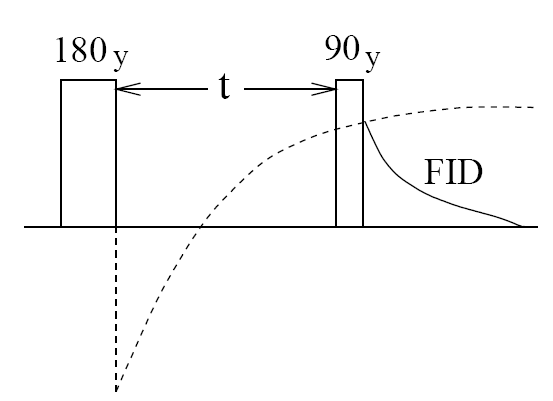
\includegraphics[width=0.5\textwidth]{images/T1_messung.png}
    \caption{Das Inversion Recovery-Experiment zur Messung der Spin-Gitter-Relaxationszeit $T_1$}
    \label{fig:T1_messung}
\end{figure}

\subsubsection{Messung von \texorpdfstring{$T_2$}{T2}}
\label{sssec:T2_Messung}

Zunächst soll das Hahn-Echo-Verfahren erklärt werden.
Dieses Verfahren nutzt die Reversibilität der Einflüsse der Feldinhomogenitäten um diese Einflüsse zu bereinigen und $T_2$ messen zu können.
Durch einen $\SI{90}{\degree}$-Puls wird der FID angeregt.
Durch einen $\SI{180}{\degree}$-Puls nach der Zeit $\tau$ werden alle Kernspin-Momente an der $y$-Achse gespiegelt. (siehe \autoref{fig:hahn_echo})
Die zuvor auseinanderlaufenden Spins laufen nun wieder aufeinander zu und so entsteht nach einer Zeit $2\tau$ ein Echo, das einen messbaren FID-Strom erzeugt.
Durch die Höhe des Echos kann die Spin-Spin-Relaxation 
\begin{equation}
    M_{x,y}(t) = M_{x,y}(t=0) \exp\left(-\frac{t}{T_2}\right)
    \label{eq:T2_relaxation}
\end{equation}
abgelesen werden. Wobei statt $t$ immer nur $2\tau$ betrachtet wird.

\begin{figure}
    \centering
    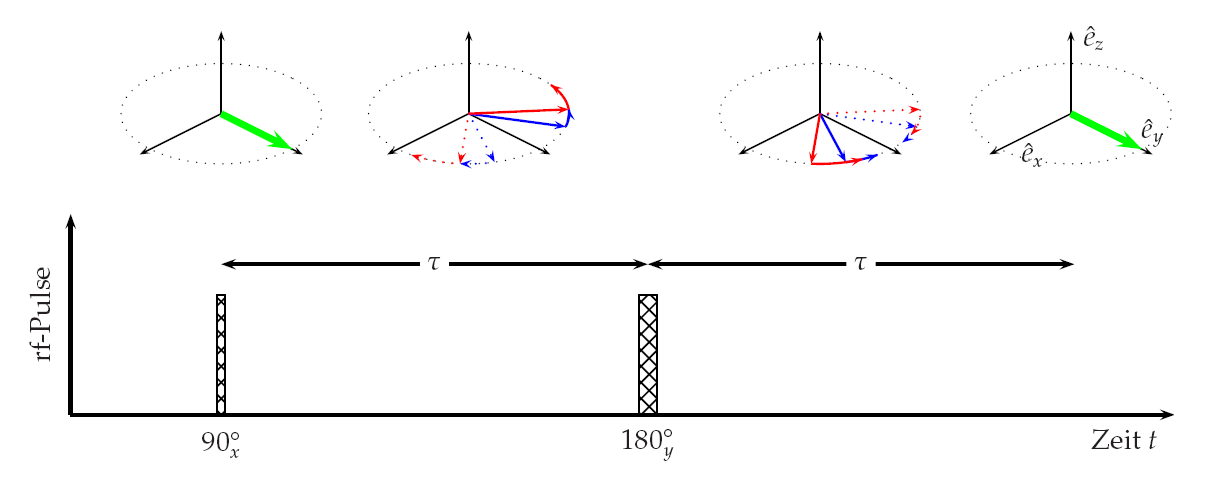
\includegraphics[width=\textwidth]{images/hahn_echo_2.png}
    \caption{Refokussierung der Magnetisierung durch ein Hahn-Echo \cite{V49}}
    \label{fig:hahn_echo}
\end{figure}

Damit nicht pro Messung nur ein Echo gemessen werden kann, wird die Hahn-Echo-Methode auf die Carr-Purcell-Methode erweitert
indem weitere $2\tau$-äquidistante $\SI{180}{\degree}$-Pulse ausgesendet werden 
und so weitere Refokussierungen und damit Echos zustande kommen.
Das Problem der Carr-Purcell-Methode ist, dass eine nicht exakte Länge des $\SI{180}{\degree}$-Pulses
dazu führt, dass die Magnetisierung nicht exakt in die $xy$-Ebene gedreht wird und so nach jedem Puls ein Fehler aufaddiert wird.

Dieses Problem wird gelöst mit der Meiboom-Gill-Methode, in der die $\SI{180}{\degree}$-Pulse um $\SI{90}{\degree}$ zu dem $\SI{90}{\degree}$-Puls ist.
So ist der Fehler in der Länge des $\SI{90}{\degree}$-Pulses egal und die Fehler der $\SI{180}{\degree}$-Pulse gleichen sich bei jedem zweiten Puls wieder aus.
Also ergibt sich hier für alle Echos bei $4n\tau$ die korrekte Amplitude und diese können verwendet werden um $T_2$ zu bestimmen.

